% !TEX encoding = UTF-8
% !TEX TS-program = pdflatex
% !TEX root = ../tesi.tex

%**************************************************************
\chapter{Protocollazione}
\label{cap:protocollazione}
%**************************************************************

\intro{Tale capitolo riporta una descrizione approfondita di cos'è un protocollo, come si deve registrare un protocollo e i possibili flussi applicativi che esso può percorrere}\\

%**************************************************************
\section{Definizione di protocollo}
La definizione di protocollo informatico, chiamato anche protocollo informatizzato, può essere tratta dal "Testo unico" in materia di documentazione amministrativa (DPR n. 445 del 28 dicembre 2000): "il legislatore ha individuato nel protocollo informatico quell'insieme di procedure informatizzate e di infrastrutture ICT (risorse di calcolo, apparati e reti di comunicazione) che le amministrazioni impiegano per la gestione documentale".
\\
\\
La protocollazione dei documenti non è intesa come mera operazione amministrativa, ma un vero e proprio procedimento amministrativo diffuso che mira alla dematerializzazione dei flussi documentali e a tutti i vantaggi che essa comporta.
Questi vantaggi, che riguardano principalmente la gestione del documento, sono:
\begin{itemize}
    \item \textbf{Flessibilità:} il documento prodotto in formato dematerializzato potrà essere corredato e completato con diverse tipologie di documenti;
    
    \item \textbf{Simulazione:} si potranno produrre infinite copie dello stesso documento conformi all'originale;
    
    \item \textbf{Conservazione:} il documento potrà essere conservato per un periodo di tempo lungo senza subire deterioramento;
    
    \item \textbf{Trasmissibilità:} il vantaggio del trasferimento dei documenti digitali è evidente;
    
    \item \textbf{Archiviazione:} grazie a determinati strumenti informatici, si può arrivare a un sistema di archiviazione e di correlazioni tra documenti che rende il loro accesso più semplice e rapido.
\end{itemize}
Un documento protocollato, dal momento della protocollazione stessa, verrà tratto sotto il profilo giuridico e gestionale.
\\
Si può quindi affermare che il protocollo è il punto di snodo di tutta la corrispondenza in entrata e in uscita di un'azienda ed è la chiave di accesso all'informazione e alla documentazione.
%**************************************************************
\section{Registrazione di un protocollo}
La registrazione di un protocollo attesta che un determinato documento è stato prodotto (arrivato, spedito o interno) in una data determinata, ha funzione giuridico-probatoria e attesta l’esistenza all'interno dell'archivio di un determinato documento.
\\
Per questo motivo le informazioni minime previste da DPR 28 dicembre 2000, n. 445 - art. 56 sono:
\begin{itemize}
    \item un codice univoco di protocollo generato automaticamente dal sistema e registrato in forma non modificabile;
    
    \item data di registrazione di protocollo assegnata automaticamente dal sistema e registrata in forma non modificabile;
    
    \item mittente per i documenti ricevuti o, in alternativa, il destinatario o i destinatari per i documenti spediti, registrati in forma non modificabile;
    
    \item oggetto del documento, registrato in forma non modificabile;
    
    \item descrizione dei documenti allegati;
    
    \item data e protocollo del documento ricevuto, se disponibili;
    
    \item l’impronta del documento informatico, se trasmesso per via telematica, costituita dalla sequenza di simboli binari in grado di identificarne univocamente il contenuto, registrata in forma non modificabile.
\end{itemize}

%**************************************************************
\section{Flusso applicativo di un protocollo}
A differenza degli “iter procedurali”, che prevedono passaggi lineari al verificarsi di una determinata condizione, il flusso digitale (\emph{workflow}\glsfirstoccur) si articola in percorsi intelligenti, definiti tenendo presente l’organigramma aziendale.
\\
Un flusso di questo tipo consente di controllare in tempo reale le fasi del ciclo esecutivo e di valutarne oggettivamente la validità, ridurre gli errori, migliorare la collaborazione e la qualità del servizio e ridurre i costi di gestione e di addestramento del personale. È possibile ridurre i costi di addestramento in quanto il software guida l'utente nei vari passaggi di gestione del protocollo.
\\
\\
Esempi di flussi documentale potrebbe essere i seguenti.
\begin{figure}[!h] 
    \centering 
    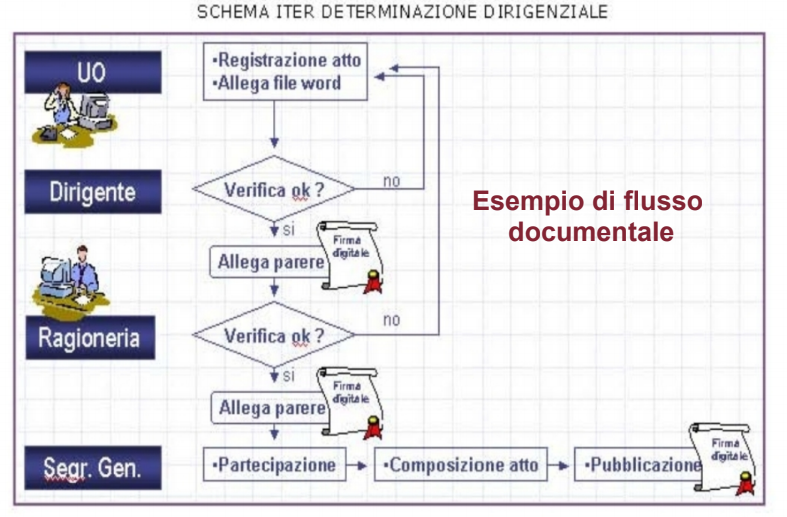
\includegraphics[width=1\columnwidth]{immagini/flussi/Flusso1.png} 
    \caption{Esempio di flusso documentale}
\end{figure}
\begin{figure}[!h] 
    \centering 
    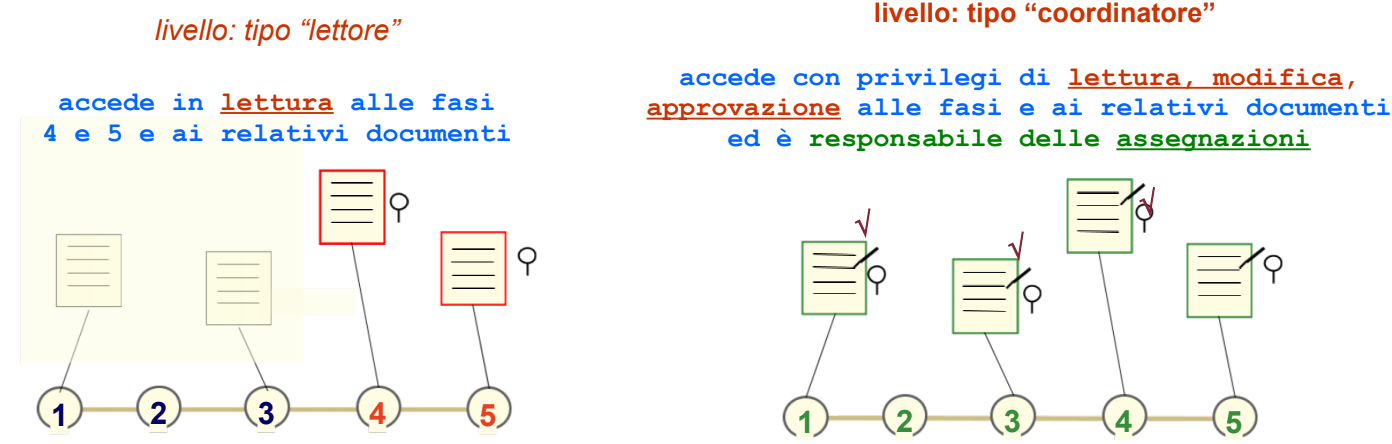
\includegraphics[width=1\columnwidth]{immagini/flussi/flusso2.png} 
    \caption{Esempio di flusso documentale}
\end{figure}
\newpage

Solo mediante il deposito di un documento elettronico in una base di dati alla
quale si attinge secondo necessità, con diverse autorizzazioni di
lettura/scrittura, è possibile gestire i flussi documentali.
\\
È quindi possibile affermare che ogni sistema di protocollazione a norma si appoggia su una piattaforma documentale.
